\documentclass[1p]{elsarticle_modified}
%\bibliographystyle{elsarticle-num}

%\usepackage[colorlinks]{hyperref}
%\usepackage{abbrmath_seonhwa} %\Abb, \Ascr, \Acal ,\Abf, \Afrak
\usepackage{amsfonts}
\usepackage{amssymb}
\usepackage{amsmath}
\usepackage{amsthm}
\usepackage{scalefnt}
\usepackage{amsbsy}
\usepackage{kotex}
\usepackage{caption}
\usepackage{subfig}
\usepackage{color}
\usepackage{graphicx}
\usepackage{xcolor} %% white, black, red, green, blue, cyan, magenta, yellow
\usepackage{float}
\usepackage{setspace}
\usepackage{hyperref}

\usepackage{tikz}
\usetikzlibrary{arrows}

\usepackage{multirow}
\usepackage{array} % fixed length table
\usepackage{hhline}

%%%%%%%%%%%%%%%%%%%%%
\makeatletter
\renewcommand*\env@matrix[1][\arraystretch]{%
	\edef\arraystretch{#1}%
	\hskip -\arraycolsep
	\let\@ifnextchar\new@ifnextchar
	\array{*\c@MaxMatrixCols c}}
\makeatother %https://tex.stackexchange.com/questions/14071/how-can-i-increase-the-line-spacing-in-a-matrix
%%%%%%%%%%%%%%%

\usepackage[normalem]{ulem}

\newcommand{\msout}[1]{\ifmmode\text{\sout{\ensuremath{#1}}}\else\sout{#1}\fi}
%SOURCE: \msout is \stkout macro in https://tex.stackexchange.com/questions/20609/strikeout-in-math-mode

\newcommand{\cancel}[1]{
	\ifmmode
	{\color{red}\msout{#1}}
	\else
	{\color{red}\sout{#1}}
	\fi
}

\newcommand{\add}[1]{
	{\color{blue}\uwave{#1}}
}

\newcommand{\replace}[2]{
	\ifmmode
	{\color{red}\msout{#1}}{\color{blue}\uwave{#2}}
	\else
	{\color{red}\sout{#1}}{\color{blue}\uwave{#2}}
	\fi
}

\newcommand{\Sol}{\mathcal{S}} %segment
\newcommand{\D}{D} %diagram
\newcommand{\A}{\mathcal{A}} %arc


%%%%%%%%%%%%%%%%%%%%%%%%%%%%%5 test

\def\sl{\operatorname{\textup{SL}}(2,\Cbb)}
\def\psl{\operatorname{\textup{PSL}}(2,\Cbb)}
\def\quan{\mkern 1mu \triangleright \mkern 1mu}

\theoremstyle{definition}
\newtheorem{thm}{Theorem}[section]
\newtheorem{prop}[thm]{Proposition}
\newtheorem{lem}[thm]{Lemma}
\newtheorem{ques}[thm]{Question}
\newtheorem{cor}[thm]{Corollary}
\newtheorem{defn}[thm]{Definition}
\newtheorem{exam}[thm]{Example}
\newtheorem{rmk}[thm]{Remark}
\newtheorem{alg}[thm]{Algorithm}

\newcommand{\I}{\sqrt{-1}}
\begin{document}

%\begin{frontmatter}
%
%\title{Boundary parabolic representations of knots up to 8 crossings}
%
%%% Group authors per affiliation:
%\author{Yunhi Cho} 
%\address{Department of Mathematics, University of Seoul, Seoul, Korea}
%\ead{yhcho@uos.ac.kr}
%
%
%\author{Seonhwa Kim} %\fnref{s_kim}}
%\address{Center for Geometry and Physics, Institute for Basic Science, Pohang, 37673, Korea}
%\ead{ryeona17@ibs.re.kr}
%
%\author{Hyuk Kim}
%\address{Department of Mathematical Sciences, Seoul National University, Seoul 08826, Korea}
%\ead{hyukkim@snu.ac.kr}
%
%\author{Seokbeom Yoon}
%\address{Department of Mathematical Sciences, Seoul National University, Seoul, 08826,  Korea}
%\ead{sbyoon15@snu.ac.kr}
%
%\begin{abstract}
%We find all boundary parabolic representation of knots up to 8 crossings.
%
%\end{abstract}
%\begin{keyword}
%    \MSC[2010] 57M25 
%\end{keyword}
%
%\end{frontmatter}

%\linenumbers
%\tableofcontents
%
\newcommand\colored[1]{\textcolor{white}{\rule[-0.35ex]{0.8em}{1.4ex}}\kern-0.8em\color{red} #1}%
%\newcommand\colored[1]{\textcolor{white}{ #1}\kern-2.17ex	\textcolor{white}{ #1}\kern-1.81ex	\textcolor{white}{ #1}\kern-2.15ex\color{red}#1	}

{\Large $\underline{12a_{0912}~(K12a_{0912})}$}

\setlength{\tabcolsep}{10pt}
\renewcommand{\arraystretch}{1.6}
\vspace{1cm}\begin{tabular}{m{100pt}>{\centering\arraybackslash}m{274pt}}
\multirow{5}{120pt}{
	\centering
	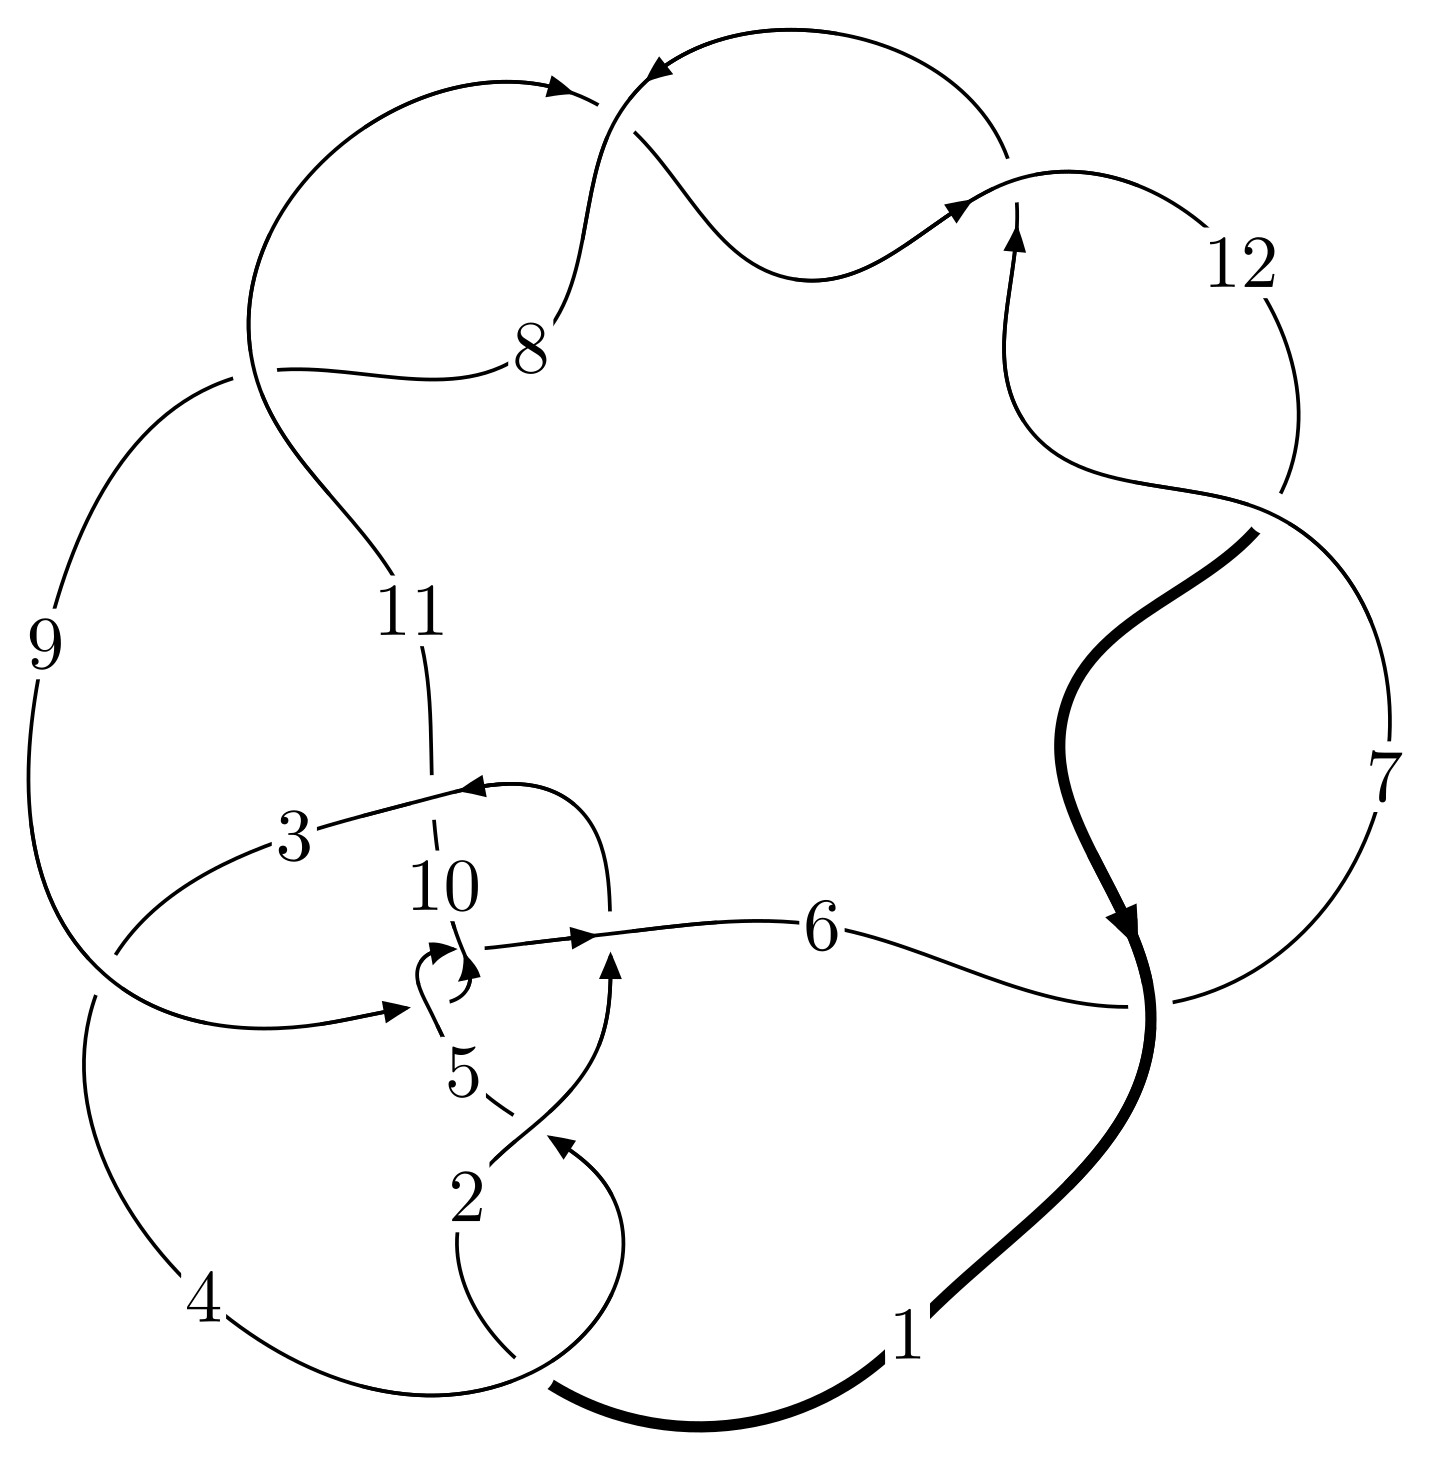
\includegraphics[width=112pt]{../../../GIT/diagram.site/Diagrams/png/1713_12a_0912.png}\\
\ \ \ A knot diagram\footnotemark}&
\allowdisplaybreaks
\textbf{Linearized knot diagam} \\
\cline{2-2}
 &
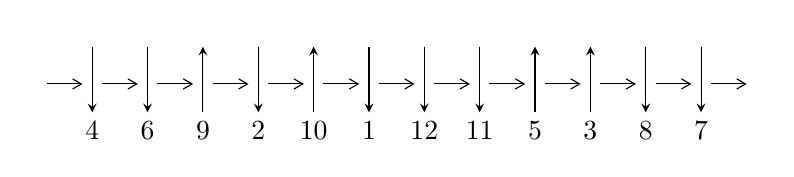
\begin{tikzpicture}[x=20pt, y=17pt]
	% nodes
	\node (C0) at (0, 0) {};
	\node (C1) at (1, 0) {};
	\node (C1U) at (1, +1) {};
	\node (C1D) at (1, -1) {4};

	\node (C2) at (2, 0) {};
	\node (C2U) at (2, +1) {};
	\node (C2D) at (2, -1) {6};

	\node (C3) at (3, 0) {};
	\node (C3U) at (3, +1) {};
	\node (C3D) at (3, -1) {9};

	\node (C4) at (4, 0) {};
	\node (C4U) at (4, +1) {};
	\node (C4D) at (4, -1) {2};

	\node (C5) at (5, 0) {};
	\node (C5U) at (5, +1) {};
	\node (C5D) at (5, -1) {10};

	\node (C6) at (6, 0) {};
	\node (C6U) at (6, +1) {};
	\node (C6D) at (6, -1) {1};

	\node (C7) at (7, 0) {};
	\node (C7U) at (7, +1) {};
	\node (C7D) at (7, -1) {12};

	\node (C8) at (8, 0) {};
	\node (C8U) at (8, +1) {};
	\node (C8D) at (8, -1) {11};

	\node (C9) at (9, 0) {};
	\node (C9U) at (9, +1) {};
	\node (C9D) at (9, -1) {5};

	\node (C10) at (10, 0) {};
	\node (C10U) at (10, +1) {};
	\node (C10D) at (10, -1) {3};

	\node (C11) at (11, 0) {};
	\node (C11U) at (11, +1) {};
	\node (C11D) at (11, -1) {8};

	\node (C12) at (12, 0) {};
	\node (C12U) at (12, +1) {};
	\node (C12D) at (12, -1) {7};
	\node (C13) at (13, 0) {};

	% arrows
	\draw[->,>={angle 60}]
	(C0) edge (C1) (C1) edge (C2) (C2) edge (C3) (C3) edge (C4) (C4) edge (C5) (C5) edge (C6) (C6) edge (C7) (C7) edge (C8) (C8) edge (C9) (C9) edge (C10) (C10) edge (C11) (C11) edge (C12) (C12) edge (C13) ;	\draw[->,>=stealth]
	(C1U) edge (C1D) (C2U) edge (C2D) (C3D) edge (C3U) (C4U) edge (C4D) (C5D) edge (C5U) (C6U) edge (C6D) (C7U) edge (C7D) (C8U) edge (C8D) (C9D) edge (C9U) (C10D) edge (C10U) (C11U) edge (C11D) (C12U) edge (C12D) ;
	\end{tikzpicture} \\
\hhline{~~} \\& 
\textbf{Solving Sequence} \\ \cline{2-2} 
 &
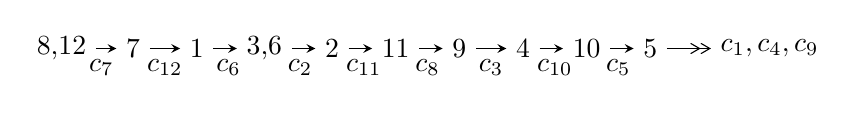
\begin{tikzpicture}[x=23pt, y=7pt]
	% node
	\node (A0) at (-1/8, 0) {8,12};
	\node (A1) at (1, 0) {7};
	\node (A2) at (2, 0) {1};
	\node (A3) at (49/16, 0) {3,6};
	\node (A4) at (33/8, 0) {2};
	\node (A5) at (41/8, 0) {11};
	\node (A6) at (49/8, 0) {9};
	\node (A7) at (57/8, 0) {4};
	\node (A8) at (65/8, 0) {10};
	\node (A9) at (73/8, 0) {5};
	\node (C1) at (1/2, -1) {$c_{7}$};
	\node (C2) at (3/2, -1) {$c_{12}$};
	\node (C3) at (5/2, -1) {$c_{6}$};
	\node (C4) at (29/8, -1) {$c_{2}$};
	\node (C5) at (37/8, -1) {$c_{11}$};
	\node (C6) at (45/8, -1) {$c_{8}$};
	\node (C7) at (53/8, -1) {$c_{3}$};
	\node (C8) at (61/8, -1) {$c_{10}$};
	\node (C9) at (69/8, -1) {$c_{5}$};
	\node (A10) at (11, 0) {$c_{1},c_{4},c_{9}$};

	% edge
	\draw[->,>=stealth]	
	(A0) edge (A1) (A1) edge (A2) (A2) edge (A3) (A3) edge (A4) (A4) edge (A5) (A5) edge (A6) (A6) edge (A7) (A7) edge (A8) (A8) edge (A9) ;
	\draw[->>,>={angle 60}]	
	(A9) edge (A10);
\end{tikzpicture} \\ 

\end{tabular} \\

\footnotetext{
The image of knot diagram is generated by the software ``\textbf{Draw programme}" developed by Andrew Bartholomew(\url{http://www.layer8.co.uk/maths/draw/index.htm\#Running-draw}), where we modified some parts for our purpose(\url{https://github.com/CATsTAILs/LinksPainter}).
}\phantom \\ \newline 
\centering \textbf{Ideals for irreducible components\footnotemark of $X_{\text{par}}$} 
 
\begin{align*}
I^u_{1}&=\langle 
-3.53538\times10^{34} u^{61}-7.35524\times10^{34} u^{60}+\cdots+5.78589\times10^{34} b-5.61888\times10^{34},\\
\phantom{I^u_{1}}&\phantom{= \langle  }-4.09242\times10^{34} u^{61}-8.12080\times10^{34} u^{60}+\cdots+5.78589\times10^{34} a-5.99085\times10^{34},\;u^{62}+2 u^{61}+\cdots+3 u+1\rangle \\
I^u_{2}&=\langle 
-5 u^3+2 u^2+8 b-9 u+3,\;-5 u^3+2 u^2+8 a-9 u+3,\;u^4- u^3+3 u^2-2 u+1\rangle \\
\\
\end{align*}
\raggedright * 2 irreducible components of $\dim_{\mathbb{C}}=0$, with total 66 representations.\\
\footnotetext{All coefficients of polynomials are rational numbers. But the coefficients are sometimes approximated in decimal forms when there is not enough margin.}
\newpage
\renewcommand{\arraystretch}{1}
\centering \section*{I. $I^u_{1}= \langle -3.54\times10^{34} u^{61}-7.36\times10^{34} u^{60}+\cdots+5.79\times10^{34} b-5.62\times10^{34},\;-4.09\times10^{34} u^{61}-8.12\times10^{34} u^{60}+\cdots+5.79\times10^{34} a-5.99\times10^{34},\;u^{62}+2 u^{61}+\cdots+3 u+1 \rangle$}
\flushleft \textbf{(i) Arc colorings}\\
\begin{tabular}{m{7pt} m{180pt} m{7pt} m{180pt} }
\flushright $a_{8}=$&$\begin{pmatrix}1\\0\end{pmatrix}$ \\
\flushright $a_{12}=$&$\begin{pmatrix}0\\u\end{pmatrix}$ \\
\flushright $a_{7}=$&$\begin{pmatrix}1\\- u^2\end{pmatrix}$ \\
\flushright $a_{1}=$&$\begin{pmatrix}- u\\u^3+u\end{pmatrix}$ \\
\flushright $a_{3}=$&$\begin{pmatrix}0.707309 u^{61}+1.40355 u^{60}+\cdots-3.00845 u+1.03542\\0.611035 u^{61}+1.27124 u^{60}+\cdots+3.64899 u+0.971135\end{pmatrix}$ \\
\flushright $a_{6}=$&$\begin{pmatrix}u^2+1\\- u^4-2 u^2\end{pmatrix}$ \\
\flushright $a_{2}=$&$\begin{pmatrix}0.977767 u^{61}+2.00250 u^{60}+\cdots-1.39856 u+1.95121\\0.326563 u^{61}+0.628916 u^{60}+\cdots+4.36630 u+1.06259\end{pmatrix}$ \\
\flushright $a_{11}=$&$\begin{pmatrix}u\\u\end{pmatrix}$ \\
\flushright $a_{9}=$&$\begin{pmatrix}u^2+1\\u^2\end{pmatrix}$ \\
\flushright $a_{4}=$&$\begin{pmatrix}1.05259 u^{61}+2.11420 u^{60}+\cdots-0.201565 u+1.91539\\0.291426 u^{61}+0.621179 u^{60}+\cdots+2.89131 u+0.940203\end{pmatrix}$ \\
\flushright $a_{10}=$&$\begin{pmatrix}-0.272512 u^{61}-0.378181 u^{60}+\cdots-1.40685 u-0.0919374\\-0.0260682 u^{61}-0.0324778 u^{60}+\cdots-2.18207 u-0.262833\end{pmatrix}$ \\
\flushright $a_{5}=$&$\begin{pmatrix}-0.272512 u^{61}-0.378181 u^{60}+\cdots-1.40685 u-0.0919374\\0.193930 u^{61}+0.304148 u^{60}+\cdots+2.41008 u+0.429675\end{pmatrix}$\\&\end{tabular}
\flushleft \textbf{(ii) Obstruction class $= -1$}\\~\\
\flushleft \textbf{(iii) Cusp Shapes $= -0.0309280 u^{61}+0.299984 u^{60}+\cdots+28.0488 u+1.88545$}\\~\\
\newpage\renewcommand{\arraystretch}{1}
\flushleft \textbf{(iv) u-Polynomials at the component}\newline \\
\begin{tabular}{m{50pt}|m{274pt}}
Crossings & \hspace{64pt}u-Polynomials at each crossing \\
\hline $$\begin{aligned}c_{1},c_{4}\end{aligned}$$&$\begin{aligned}
&u^{62}-5 u^{61}+\cdots-321 u+64
\end{aligned}$\\
\hline $$\begin{aligned}c_{2}\end{aligned}$$&$\begin{aligned}
&8(8 u^{62}-57 u^{61}+\cdots-5508 u+7609)
\end{aligned}$\\
\hline $$\begin{aligned}c_{3}\end{aligned}$$&$\begin{aligned}
&8(8 u^{62}-21 u^{61}+\cdots+2370 u+179)
\end{aligned}$\\
\hline $$\begin{aligned}c_{5},c_{9}\end{aligned}$$&$\begin{aligned}
&u^{62}+2 u^{61}+\cdots+3 u+1
\end{aligned}$\\
\hline $$\begin{aligned}c_{6},c_{7},c_{8}\\c_{11},c_{12}\end{aligned}$$&$\begin{aligned}
&u^{62}-2 u^{61}+\cdots-3 u+1
\end{aligned}$\\
\hline $$\begin{aligned}c_{10}\end{aligned}$$&$\begin{aligned}
&u^{62}+3 u^{61}+\cdots+2496 u+1024
\end{aligned}$\\
\hline
\end{tabular}\\~\\
\newpage\renewcommand{\arraystretch}{1}
\flushleft \textbf{(v) Riley Polynomials at the component}\newline \\
\begin{tabular}{m{50pt}|m{274pt}}
Crossings & \hspace{64pt}Riley Polynomials at each crossing \\
\hline $$\begin{aligned}c_{1},c_{4}\end{aligned}$$&$\begin{aligned}
&y^{62}-31 y^{61}+\cdots+34687 y+4096
\end{aligned}$\\
\hline $$\begin{aligned}c_{2}\end{aligned}$$&$\begin{aligned}
&64(64 y^{62}+223 y^{61}+\cdots+7.95786\times10^{8} y+5.78969\times10^{7})
\end{aligned}$\\
\hline $$\begin{aligned}c_{3}\end{aligned}$$&$\begin{aligned}
&64(64 y^{62}-2857 y^{61}+\cdots-2988464 y+32041)
\end{aligned}$\\
\hline $$\begin{aligned}c_{5},c_{9}\end{aligned}$$&$\begin{aligned}
&y^{62}-34 y^{61}+\cdots-5 y+1
\end{aligned}$\\
\hline $$\begin{aligned}c_{6},c_{7},c_{8}\\c_{11},c_{12}\end{aligned}$$&$\begin{aligned}
&y^{62}+82 y^{61}+\cdots-5 y+1
\end{aligned}$\\
\hline $$\begin{aligned}c_{10}\end{aligned}$$&$\begin{aligned}
&y^{62}-27 y^{61}+\cdots-9949184 y+1048576
\end{aligned}$\\
\hline
\end{tabular}\\~\\
\newpage\flushleft \textbf{(vi) Complex Volumes and Cusp Shapes}
$$\begin{array}{c|c|c}  
\text{Solutions to }I^u_{1}& \I (\text{vol} + \sqrt{-1}CS) & \text{Cusp shape}\\
 \hline 
\begin{aligned}
u &= \phantom{-}0.070453 + 1.008300 I \\
a &= \phantom{-}2.41201 - 2.05029 I \\
b &= \phantom{-}1.89323 - 2.09210 I\end{aligned}
 & \phantom{-}3.75467 + 0.00521 I & \phantom{-0.000000 } 0 \\ \hline\begin{aligned}
u &= \phantom{-}0.070453 - 1.008300 I \\
a &= \phantom{-}2.41201 + 2.05029 I \\
b &= \phantom{-}1.89323 + 2.09210 I\end{aligned}
 & \phantom{-}3.75467 - 0.00521 I & \phantom{-0.000000 } 0 \\ \hline\begin{aligned}
u &= \phantom{-}0.181790 + 0.945505 I \\
a &= \phantom{-}0.482726 - 0.006483 I \\
b &= -1.190670 - 0.035089 I\end{aligned}
 & \phantom{-}2.30320 - 4.63639 I & \phantom{-0.000000 } 0 \\ \hline\begin{aligned}
u &= \phantom{-}0.181790 - 0.945505 I \\
a &= \phantom{-}0.482726 + 0.006483 I \\
b &= -1.190670 + 0.035089 I\end{aligned}
 & \phantom{-}2.30320 + 4.63639 I & \phantom{-0.000000 } 0 \\ \hline\begin{aligned}
u &= -0.329924 + 1.002430 I \\
a &= \phantom{-}0.681675 + 0.062269 I \\
b &= \phantom{-}0.920280 + 1.043650 I\end{aligned}
 & \phantom{-}7.11283 + 2.06836 I & \phantom{-0.000000 } 0 \\ \hline\begin{aligned}
u &= -0.329924 - 1.002430 I \\
a &= \phantom{-}0.681675 - 0.062269 I \\
b &= \phantom{-}0.920280 - 1.043650 I\end{aligned}
 & \phantom{-}7.11283 - 2.06836 I & \phantom{-0.000000 } 0 \\ \hline\begin{aligned}
u &= -0.110698 + 0.915218 I \\
a &= -0.906019 + 0.382288 I \\
b &= \phantom{-}0.097013 + 0.988332 I\end{aligned}
 & \phantom{-}0.59146 + 1.40911 I & \phantom{-0.000000 } 0 \\ \hline\begin{aligned}
u &= -0.110698 - 0.915218 I \\
a &= -0.906019 - 0.382288 I \\
b &= \phantom{-}0.097013 - 0.988332 I\end{aligned}
 & \phantom{-}0.59146 - 1.40911 I & \phantom{-0.000000 } 0 \\ \hline\begin{aligned}
u &= -0.241171 + 1.079550 I \\
a &= -0.263274 - 0.708351 I \\
b &= \phantom{-}0.13064 - 2.22317 I\end{aligned}
 & \phantom{-}8.23800 + 6.15877 I & \phantom{-0.000000 } 0 \\ \hline\begin{aligned}
u &= -0.241171 - 1.079550 I \\
a &= -0.263274 + 0.708351 I \\
b &= \phantom{-}0.13064 + 2.22317 I\end{aligned}
 & \phantom{-}8.23800 - 6.15877 I & \phantom{-0.000000 } 0\\
 \hline 
 \end{array}$$\newpage$$\begin{array}{c|c|c}  
\text{Solutions to }I^u_{1}& \I (\text{vol} + \sqrt{-1}CS) & \text{Cusp shape}\\
 \hline 
\begin{aligned}
u &= \phantom{-}0.173893 + 1.094910 I \\
a &= \phantom{-}0.307305 - 0.647520 I \\
b &= -0.05498 - 1.49102 I\end{aligned}
 & \phantom{-}4.39365 - 2.33302 I & \phantom{-0.000000 } 0 \\ \hline\begin{aligned}
u &= \phantom{-}0.173893 - 1.094910 I \\
a &= \phantom{-}0.307305 + 0.647520 I \\
b &= -0.05498 + 1.49102 I\end{aligned}
 & \phantom{-}4.39365 + 2.33302 I & \phantom{-0.000000 } 0 \\ \hline\begin{aligned}
u &= \phantom{-}0.382128 + 1.060710 I \\
a &= -0.283114 + 0.498733 I \\
b &= -0.05935 + 1.53726 I\end{aligned}
 & \phantom{-}1.82629 - 6.88277 I & \phantom{-0.000000 } 0 \\ \hline\begin{aligned}
u &= \phantom{-}0.382128 - 1.060710 I \\
a &= -0.283114 - 0.498733 I \\
b &= -0.05935 - 1.53726 I\end{aligned}
 & \phantom{-}1.82629 + 6.88277 I & \phantom{-0.000000 } 0 \\ \hline\begin{aligned}
u &= -0.360863 + 1.083000 I \\
a &= \phantom{-}0.340097 + 0.839627 I \\
b &= \phantom{-}0.00161 + 2.17450 I\end{aligned}
 & \phantom{-}5.31778 + 12.69260 I & \phantom{-0.000000 } 0 \\ \hline\begin{aligned}
u &= -0.360863 - 1.083000 I \\
a &= \phantom{-}0.340097 - 0.839627 I \\
b &= \phantom{-}0.00161 - 2.17450 I\end{aligned}
 & \phantom{-}5.31778 - 12.69260 I & \phantom{-0.000000 } 0 \\ \hline\begin{aligned}
u &= -0.069609 + 0.834401 I \\
a &= -0.397322 + 0.616061 I \\
b &= \phantom{-}0.22387 + 2.04792 I\end{aligned}
 & \phantom{-}0.09233 + 1.48715 I & -2.19079 - 3.99799 I \\ \hline\begin{aligned}
u &= -0.069609 - 0.834401 I \\
a &= -0.397322 - 0.616061 I \\
b &= \phantom{-}0.22387 - 2.04792 I\end{aligned}
 & \phantom{-}0.09233 - 1.48715 I & -2.19079 + 3.99799 I \\ \hline\begin{aligned}
u &= \phantom{-}0.563401 + 0.581571 I \\
a &= \phantom{-}0.434752 - 0.199850 I \\
b &= -0.325684 + 0.214730 I\end{aligned}
 & -1.30352 - 0.70213 I & \phantom{-}1.08488 - 2.08211 I \\ \hline\begin{aligned}
u &= \phantom{-}0.563401 - 0.581571 I \\
a &= \phantom{-}0.434752 + 0.199850 I \\
b &= -0.325684 - 0.214730 I\end{aligned}
 & -1.30352 + 0.70213 I & \phantom{-}1.08488 + 2.08211 I\\
 \hline 
 \end{array}$$\newpage$$\begin{array}{c|c|c}  
\text{Solutions to }I^u_{1}& \I (\text{vol} + \sqrt{-1}CS) & \text{Cusp shape}\\
 \hline 
\begin{aligned}
u &= -0.255043 + 1.200940 I \\
a &= -0.401233 - 0.467101 I \\
b &= -0.76852 - 1.23254 I\end{aligned}
 & \phantom{-}6.76138 - 2.45433 I & \phantom{-0.000000 } 0 \\ \hline\begin{aligned}
u &= -0.255043 - 1.200940 I \\
a &= -0.401233 + 0.467101 I \\
b &= -0.76852 + 1.23254 I\end{aligned}
 & \phantom{-}6.76138 + 2.45433 I & \phantom{-0.000000 } 0 \\ \hline\begin{aligned}
u &= -0.583913 + 0.454618 I \\
a &= -1.048110 - 0.044724 I \\
b &= \phantom{-}0.526648 + 0.216745 I\end{aligned}
 & \phantom{-}1.44700 - 5.36748 I & -1.39491 + 3.36000 I \\ \hline\begin{aligned}
u &= -0.583913 - 0.454618 I \\
a &= -1.048110 + 0.044724 I \\
b &= \phantom{-}0.526648 - 0.216745 I\end{aligned}
 & \phantom{-}1.44700 + 5.36748 I & -1.39491 - 3.36000 I \\ \hline\begin{aligned}
u &= \phantom{-}0.658726 + 0.253626 I \\
a &= -0.656410 + 0.567952 I \\
b &= \phantom{-}0.180230 - 0.443043 I\end{aligned}
 & -2.25995 - 3.35953 I & -4.38672 + 6.99367 I \\ \hline\begin{aligned}
u &= \phantom{-}0.658726 - 0.253626 I \\
a &= -0.656410 - 0.567952 I \\
b &= \phantom{-}0.180230 + 0.443043 I\end{aligned}
 & -2.25995 + 3.35953 I & -4.38672 - 6.99367 I \\ \hline\begin{aligned}
u &= -0.627368 + 0.304568 I \\
a &= \phantom{-}0.877042 + 0.926675 I \\
b &= -0.155103 - 0.758475 I\end{aligned}
 & \phantom{-}0.99678 + 9.33410 I & -2.66606 - 8.39608 I \\ \hline\begin{aligned}
u &= -0.627368 - 0.304568 I \\
a &= \phantom{-}0.877042 - 0.926675 I \\
b &= -0.155103 + 0.758475 I\end{aligned}
 & \phantom{-}0.99678 - 9.33410 I & -2.66606 + 8.39608 I \\ \hline\begin{aligned}
u &= -0.448611 + 0.353688 I \\
a &= -0.63018 - 1.63885 I \\
b &= \phantom{-}0.263806 + 0.539972 I\end{aligned}
 & \phantom{-}3.76404 + 3.80466 I & \phantom{-}0.97266 - 6.48808 I \\ \hline\begin{aligned}
u &= -0.448611 - 0.353688 I \\
a &= -0.63018 + 1.63885 I \\
b &= \phantom{-}0.263806 - 0.539972 I\end{aligned}
 & \phantom{-}3.76404 - 3.80466 I & \phantom{-}0.97266 + 6.48808 I\\
 \hline 
 \end{array}$$\newpage$$\begin{array}{c|c|c}  
\text{Solutions to }I^u_{1}& \I (\text{vol} + \sqrt{-1}CS) & \text{Cusp shape}\\
 \hline 
\begin{aligned}
u &= -0.497757 + 0.225969 I \\
a &= \phantom{-}1.063150 + 0.042781 I \\
b &= -0.742489 - 0.206163 I\end{aligned}
 & \phantom{-}3.37167 - 0.77892 I & \phantom{-}0.45056 - 2.40505 I \\ \hline\begin{aligned}
u &= -0.497757 - 0.225969 I \\
a &= \phantom{-}1.063150 - 0.042781 I \\
b &= -0.742489 + 0.206163 I\end{aligned}
 & \phantom{-}3.37167 + 0.77892 I & \phantom{-}0.45056 + 2.40505 I \\ \hline\begin{aligned}
u &= \phantom{-}0.14026 + 1.52029 I \\
a &= \phantom{-}0.109842 - 0.293520 I \\
b &= \phantom{-}0.136239 - 0.648021 I\end{aligned}
 & \phantom{-}5.58374 - 3.21684 I & \phantom{-0.000000 } 0 \\ \hline\begin{aligned}
u &= \phantom{-}0.14026 - 1.52029 I \\
a &= \phantom{-}0.109842 + 0.293520 I \\
b &= \phantom{-}0.136239 + 0.648021 I\end{aligned}
 & \phantom{-}5.58374 + 3.21684 I & \phantom{-0.000000 } 0 \\ \hline\begin{aligned}
u &= \phantom{-}0.382370 + 0.144909 I \\
a &= -2.29821 - 1.74988 I \\
b &= -0.105131 + 0.442226 I\end{aligned}
 & -1.00840 - 2.70031 I & -7.30327 + 8.03455 I \\ \hline\begin{aligned}
u &= \phantom{-}0.382370 - 0.144909 I \\
a &= -2.29821 + 1.74988 I \\
b &= -0.105131 - 0.442226 I\end{aligned}
 & -1.00840 + 2.70031 I & -7.30327 - 8.03455 I \\ \hline\begin{aligned}
u &= \phantom{-}0.257995 + 0.303118 I \\
a &= -0.360406 - 0.861445 I \\
b &= -0.005399 + 0.393666 I\end{aligned}
 & -0.107004 - 0.841367 I & -2.66690 + 7.99137 I \\ \hline\begin{aligned}
u &= \phantom{-}0.257995 - 0.303118 I \\
a &= -0.360406 + 0.861445 I \\
b &= -0.005399 - 0.393666 I\end{aligned}
 & -0.107004 + 0.841367 I & -2.66690 - 7.99137 I \\ \hline\begin{aligned}
u &= \phantom{-}0.171710 + 0.316302 I \\
a &= -0.600051 - 0.117965 I \\
b &= \phantom{-}0.29575 + 1.66039 I\end{aligned}
 & -0.194780 + 0.812413 I & \phantom{-}0.93566 + 8.09045 I \\ \hline\begin{aligned}
u &= \phantom{-}0.171710 - 0.316302 I \\
a &= -0.600051 + 0.117965 I \\
b &= \phantom{-}0.29575 - 1.66039 I\end{aligned}
 & -0.194780 - 0.812413 I & \phantom{-}0.93566 - 8.09045 I\\
 \hline 
 \end{array}$$\newpage$$\begin{array}{c|c|c}  
\text{Solutions to }I^u_{1}& \I (\text{vol} + \sqrt{-1}CS) & \text{Cusp shape}\\
 \hline 
\begin{aligned}
u &= -0.324588 + 0.004379 I \\
a &= \phantom{-}2.89984 - 0.03792 I \\
b &= \phantom{-}0.408718 + 0.019164 I\end{aligned}
 & -2.18849 + 0.0001 I & -8.36748 + 0.29865 I \\ \hline\begin{aligned}
u &= -0.324588 - 0.004379 I \\
a &= \phantom{-}2.89984 + 0.03792 I \\
b &= \phantom{-}0.408718 - 0.019164 I\end{aligned}
 & -2.18849 - 0.0001 I & -8.36748 - 0.29865 I \\ \hline\begin{aligned}
u &= -0.00897 + 1.69781 I \\
a &= -0.39272 - 3.11626 I \\
b &= -0.72887 - 4.08987 I\end{aligned}
 & \phantom{-}9.22742 + 1.71660 I & \phantom{-0.000000 } 0 \\ \hline\begin{aligned}
u &= -0.00897 - 1.69781 I \\
a &= -0.39272 + 3.11626 I \\
b &= -0.72887 + 4.08987 I\end{aligned}
 & \phantom{-}9.22742 - 1.71660 I & \phantom{-0.000000 } 0 \\ \hline\begin{aligned}
u &= -0.02316 + 1.70966 I \\
a &= -0.43712 - 1.36309 I \\
b &= -1.14797 - 1.80302 I\end{aligned}
 & \phantom{-}10.01640 + 1.89978 I & \phantom{-0.000000 } 0 \\ \hline\begin{aligned}
u &= -0.02316 - 1.70966 I \\
a &= -0.43712 + 1.36309 I \\
b &= -1.14797 + 1.80302 I\end{aligned}
 & \phantom{-}10.01640 - 1.89978 I & \phantom{-0.000000 } 0 \\ \hline\begin{aligned}
u &= \phantom{-}0.03865 + 1.71177 I \\
a &= \phantom{-}1.64069 + 0.08478 I \\
b &= \phantom{-}2.76769 + 0.00130 I\end{aligned}
 & \phantom{-}11.79830 - 5.46026 I & \phantom{-0.000000 } 0 \\ \hline\begin{aligned}
u &= \phantom{-}0.03865 - 1.71177 I \\
a &= \phantom{-}1.64069 - 0.08478 I \\
b &= \phantom{-}2.76769 - 0.00130 I\end{aligned}
 & \phantom{-}11.79830 + 5.46026 I & \phantom{-0.000000 } 0 \\ \hline\begin{aligned}
u &= -0.09249 + 1.72353 I \\
a &= -1.00407 - 1.43069 I \\
b &= -0.84968 - 2.10785 I\end{aligned}
 & \phantom{-}16.7807 + 3.8111 I & \phantom{-0.000000 } 0 \\ \hline\begin{aligned}
u &= -0.09249 - 1.72353 I \\
a &= -1.00407 + 1.43069 I \\
b &= -0.84968 + 2.10785 I\end{aligned}
 & \phantom{-}16.7807 - 3.8111 I & \phantom{-0.000000 } 0\\
 \hline 
 \end{array}$$\newpage$$\begin{array}{c|c|c}  
\text{Solutions to }I^u_{1}& \I (\text{vol} + \sqrt{-1}CS) & \text{Cusp shape}\\
 \hline 
\begin{aligned}
u &= \phantom{-}0.01534 + 1.72861 I \\
a &= -3.06068 + 1.08280 I \\
b &= -2.72644 + 1.01992 I\end{aligned}
 & \phantom{-}13.59990 - 0.32504 I & \phantom{-0.000000 } 0 \\ \hline\begin{aligned}
u &= \phantom{-}0.01534 - 1.72861 I \\
a &= -3.06068 - 1.08280 I \\
b &= -2.72644 - 1.01992 I\end{aligned}
 & \phantom{-}13.59990 + 0.32504 I & \phantom{-0.000000 } 0 \\ \hline\begin{aligned}
u &= \phantom{-}0.10151 + 1.73858 I \\
a &= \phantom{-}0.30042 - 2.09901 I \\
b &= -0.09887 - 2.80202 I\end{aligned}
 & \phantom{-}11.7585 - 8.8832 I & \phantom{-0.000000 } 0 \\ \hline\begin{aligned}
u &= \phantom{-}0.10151 - 1.73858 I \\
a &= \phantom{-}0.30042 + 2.09901 I \\
b &= -0.09887 + 2.80202 I\end{aligned}
 & \phantom{-}11.7585 + 8.8832 I & \phantom{-0.000000 } 0 \\ \hline\begin{aligned}
u &= -0.06180 + 1.74280 I \\
a &= \phantom{-}0.02606 + 2.99792 I \\
b &= -0.42662 + 4.03827 I\end{aligned}
 & \phantom{-}18.3544 + 7.4189 I & \phantom{-0.000000 } 0 \\ \hline\begin{aligned}
u &= -0.06180 - 1.74280 I \\
a &= \phantom{-}0.02606 - 2.99792 I \\
b &= -0.42662 - 4.03827 I\end{aligned}
 & \phantom{-}18.3544 - 7.4189 I & \phantom{-0.000000 } 0 \\ \hline\begin{aligned}
u &= -0.09644 + 1.74449 I \\
a &= -0.35373 - 2.76349 I \\
b &= \phantom{-}0.12777 - 3.62070 I\end{aligned}
 & \phantom{-}15.3794 + 14.6067 I & \phantom{-0.000000 } 0 \\ \hline\begin{aligned}
u &= -0.09644 - 1.74449 I \\
a &= -0.35373 + 2.76349 I \\
b &= \phantom{-}0.12777 + 3.62070 I\end{aligned}
 & \phantom{-}15.3794 - 14.6067 I & \phantom{-0.000000 } 0 \\ \hline\begin{aligned}
u &= \phantom{-}0.04860 + 1.74694 I \\
a &= -0.05763 + 2.17932 I \\
b &= \phantom{-}0.31904 + 2.84558 I\end{aligned}
 & \phantom{-}14.6212 - 3.2967 I & \phantom{-0.000000 } 0 \\ \hline\begin{aligned}
u &= \phantom{-}0.04860 - 1.74694 I \\
a &= -0.05763 - 2.17932 I \\
b &= \phantom{-}0.31904 - 2.84558 I\end{aligned}
 & \phantom{-}14.6212 + 3.2967 I & \phantom{-0.000000 } 0\\
 \hline 
 \end{array}$$\newpage$$\begin{array}{c|c|c}  
\text{Solutions to }I^u_{1}& \I (\text{vol} + \sqrt{-1}CS) & \text{Cusp shape}\\
 \hline 
\begin{aligned}
u &= -0.05441 + 1.76916 I \\
a &= \phantom{-}0.76218 + 1.84328 I \\
b &= \phantom{-}0.78075 + 2.48268 I\end{aligned}
 & \phantom{-}17.4935 - 1.1900 I & \phantom{-0.000000 } 0 \\ \hline\begin{aligned}
u &= -0.05441 - 1.76916 I \\
a &= \phantom{-}0.76218 - 1.84328 I \\
b &= \phantom{-}0.78075 - 2.48268 I\end{aligned}
 & \phantom{-}17.4935 + 1.1900 I & \phantom{-0.000000 } 0\\
 \hline 
 \end{array}$$\newpage\newpage\renewcommand{\arraystretch}{1}
\centering \section*{II. $I^u_{2}= \langle -5 u^3+2 u^2+8 b-9 u+3,\;-5 u^3+2 u^2+8 a-9 u+3,\;u^4- u^3+3 u^2-2 u+1 \rangle$}
\flushleft \textbf{(i) Arc colorings}\\
\begin{tabular}{m{7pt} m{180pt} m{7pt} m{180pt} }
\flushright $a_{8}=$&$\begin{pmatrix}1\\0\end{pmatrix}$ \\
\flushright $a_{12}=$&$\begin{pmatrix}0\\u\end{pmatrix}$ \\
\flushright $a_{7}=$&$\begin{pmatrix}1\\- u^2\end{pmatrix}$ \\
\flushright $a_{1}=$&$\begin{pmatrix}- u\\u^3+u\end{pmatrix}$ \\
\flushright $a_{3}=$&$\begin{pmatrix}\frac{5}{8} u^3-\frac{1}{4} u^2+\frac{9}{8} u-\frac{3}{8}\\\frac{5}{8} u^3-\frac{1}{4} u^2+\frac{9}{8} u-\frac{3}{8}\end{pmatrix}$ \\
\flushright $a_{6}=$&$\begin{pmatrix}u^2+1\\- u^3+u^2-2 u+1\end{pmatrix}$ \\
\flushright $a_{2}=$&$\begin{pmatrix}\frac{7}{8} u^3-\frac{3}{4} u^2+\frac{11}{8} u-\frac{9}{8}\\\frac{5}{4} u^3-\frac{1}{2} u^2+\frac{9}{4} u-\frac{3}{4}\end{pmatrix}$ \\
\flushright $a_{11}=$&$\begin{pmatrix}u\\u\end{pmatrix}$ \\
\flushright $a_{9}=$&$\begin{pmatrix}u^2+1\\u^2\end{pmatrix}$ \\
\flushright $a_{4}=$&$\begin{pmatrix}\frac{7}{8} u^3-\frac{3}{4} u^2+\frac{19}{8} u-\frac{9}{8}\\\frac{1}{4} u^3-\frac{1}{2} u^2+\frac{5}{4} u-\frac{3}{4}\end{pmatrix}$ \\
\flushright $a_{10}=$&$\begin{pmatrix}u\\u\end{pmatrix}$ \\
\flushright $a_{5}=$&$\begin{pmatrix}u\\- u^3- u\end{pmatrix}$\\&\end{tabular}
\flushleft \textbf{(ii) Obstruction class $= 1$}\\~\\
\flushleft \textbf{(iii) Cusp Shapes $= \frac{279}{64} u^3-\frac{51}{32} u^2+\frac{731}{64} u-\frac{609}{64}$}\\~\\
\newpage\renewcommand{\arraystretch}{1}
\flushleft \textbf{(iv) u-Polynomials at the component}\newline \\
\begin{tabular}{m{50pt}|m{274pt}}
Crossings & \hspace{64pt}u-Polynomials at each crossing \\
\hline $$\begin{aligned}c_{1}\end{aligned}$$&$\begin{aligned}
&(u-1)^4
\end{aligned}$\\
\hline $$\begin{aligned}c_{2}\end{aligned}$$&$\begin{aligned}
&8(8 u^4-15 u^3+12 u^2-5 u+1)
\end{aligned}$\\
\hline $$\begin{aligned}c_{3}\end{aligned}$$&$\begin{aligned}
&8(8 u^4-3 u^3+6 u^2- u+1)
\end{aligned}$\\
\hline $$\begin{aligned}c_{4}\end{aligned}$$&$\begin{aligned}
&(u+1)^4
\end{aligned}$\\
\hline $$\begin{aligned}c_{5}\end{aligned}$$&$\begin{aligned}
&u^4- u^3+u^2+1
\end{aligned}$\\
\hline $$\begin{aligned}c_{6},c_{7},c_{8}\end{aligned}$$&$\begin{aligned}
&u^4- u^3+3 u^2-2 u+1
\end{aligned}$\\
\hline $$\begin{aligned}c_{9}\end{aligned}$$&$\begin{aligned}
&u^4+u^3+u^2+1
\end{aligned}$\\
\hline $$\begin{aligned}c_{10}\end{aligned}$$&$\begin{aligned}
&u^4
\end{aligned}$\\
\hline $$\begin{aligned}c_{11},c_{12}\end{aligned}$$&$\begin{aligned}
&u^4+u^3+3 u^2+2 u+1
\end{aligned}$\\
\hline
\end{tabular}\\~\\
\newpage\renewcommand{\arraystretch}{1}
\flushleft \textbf{(v) Riley Polynomials at the component}\newline \\
\begin{tabular}{m{50pt}|m{274pt}}
Crossings & \hspace{64pt}Riley Polynomials at each crossing \\
\hline $$\begin{aligned}c_{1},c_{4}\end{aligned}$$&$\begin{aligned}
&(y-1)^4
\end{aligned}$\\
\hline $$\begin{aligned}c_{2}\end{aligned}$$&$\begin{aligned}
&64(64 y^4-33 y^3+10 y^2- y+1)
\end{aligned}$\\
\hline $$\begin{aligned}c_{3}\end{aligned}$$&$\begin{aligned}
&64(64 y^4+87 y^3+46 y^2+11 y+1)
\end{aligned}$\\
\hline $$\begin{aligned}c_{5},c_{9}\end{aligned}$$&$\begin{aligned}
&y^4+y^3+3 y^2+2 y+1
\end{aligned}$\\
\hline $$\begin{aligned}c_{6},c_{7},c_{8}\\c_{11},c_{12}\end{aligned}$$&$\begin{aligned}
&y^4+5 y^3+7 y^2+2 y+1
\end{aligned}$\\
\hline $$\begin{aligned}c_{10}\end{aligned}$$&$\begin{aligned}
&y^4
\end{aligned}$\\
\hline
\end{tabular}\\~\\
\newpage\flushleft \textbf{(vi) Complex Volumes and Cusp Shapes}
$$\begin{array}{c|c|c}  
\text{Solutions to }I^u_{2}& \I (\text{vol} + \sqrt{-1}CS) & \text{Cusp shape}\\
 \hline 
\begin{aligned}
u &= \phantom{-}0.395123 + 0.506844 I \\
a &= -0.057058 + 0.537058 I \\
b &= -0.057058 + 0.537058 I\end{aligned}
 & -1.85594 - 1.41510 I & -5.90053 + 5.61802 I \\ \hline\begin{aligned}
u &= \phantom{-}0.395123 - 0.506844 I \\
a &= -0.057058 - 0.537058 I \\
b &= -0.057058 - 0.537058 I\end{aligned}
 & -1.85594 + 1.41510 I & -5.90053 - 5.61802 I \\ \hline\begin{aligned}
u &= \phantom{-}0.10488 + 1.55249 I \\
a &= -0.130442 - 0.641504 I \\
b &= -0.130442 - 0.641504 I\end{aligned}
 & \phantom{-}5.14581 - 3.16396 I & -7.79478 + 1.12451 I \\ \hline\begin{aligned}
u &= \phantom{-}0.10488 - 1.55249 I \\
a &= -0.130442 + 0.641504 I \\
b &= -0.130442 + 0.641504 I\end{aligned}
 & \phantom{-}5.14581 + 3.16396 I & -7.79478 - 1.12451 I\\
 \hline 
 \end{array}$$\newpage
\newpage\renewcommand{\arraystretch}{1}
\centering \section*{ III. u-Polynomials}
\begin{tabular}{m{50pt}|m{274pt}}
Crossings & \hspace{64pt}u-Polynomials at each crossing \\
\hline $$\begin{aligned}c_{1}\end{aligned}$$&$\begin{aligned}
&((u-1)^4)(u^{62}-5 u^{61}+\cdots-321 u+64)
\end{aligned}$\\
\hline $$\begin{aligned}c_{2}\end{aligned}$$&$\begin{aligned}
&64(8 u^4-15 u^3+\cdots-5 u+1)(8 u^{62}-57 u^{61}+\cdots-5508 u+7609)
\end{aligned}$\\
\hline $$\begin{aligned}c_{3}\end{aligned}$$&$\begin{aligned}
&64(8 u^4-3 u^3+\cdots- u+1)(8 u^{62}-21 u^{61}+\cdots+2370 u+179)
\end{aligned}$\\
\hline $$\begin{aligned}c_{4}\end{aligned}$$&$\begin{aligned}
&((u+1)^4)(u^{62}-5 u^{61}+\cdots-321 u+64)
\end{aligned}$\\
\hline $$\begin{aligned}c_{5}\end{aligned}$$&$\begin{aligned}
&(u^4- u^3+u^2+1)(u^{62}+2 u^{61}+\cdots+3 u+1)
\end{aligned}$\\
\hline $$\begin{aligned}c_{6},c_{7},c_{8}\end{aligned}$$&$\begin{aligned}
&(u^4- u^3+3 u^2-2 u+1)(u^{62}-2 u^{61}+\cdots-3 u+1)
\end{aligned}$\\
\hline $$\begin{aligned}c_{9}\end{aligned}$$&$\begin{aligned}
&(u^4+u^3+u^2+1)(u^{62}+2 u^{61}+\cdots+3 u+1)
\end{aligned}$\\
\hline $$\begin{aligned}c_{10}\end{aligned}$$&$\begin{aligned}
&u^4(u^{62}+3 u^{61}+\cdots+2496 u+1024)
\end{aligned}$\\
\hline $$\begin{aligned}c_{11},c_{12}\end{aligned}$$&$\begin{aligned}
&(u^4+u^3+3 u^2+2 u+1)(u^{62}-2 u^{61}+\cdots-3 u+1)
\end{aligned}$\\
\hline
\end{tabular}\newpage\renewcommand{\arraystretch}{1}
\centering \section*{ IV. Riley Polynomials}
\begin{tabular}{m{50pt}|m{274pt}}
Crossings & \hspace{64pt}Riley Polynomials at each crossing \\
\hline $$\begin{aligned}c_{1},c_{4}\end{aligned}$$&$\begin{aligned}
&((y-1)^4)(y^{62}-31 y^{61}+\cdots+34687 y+4096)
\end{aligned}$\\
\hline $$\begin{aligned}c_{2}\end{aligned}$$&$\begin{aligned}
&4096(64 y^4-33 y^3+10 y^2- y+1)\\
&\cdot(64 y^{62}+223 y^{61}+\cdots+795786284 y+57896881)
\end{aligned}$\\
\hline $$\begin{aligned}c_{3}\end{aligned}$$&$\begin{aligned}
&4096(64 y^4+87 y^3+46 y^2+11 y+1)\\
&\cdot(64 y^{62}-2857 y^{61}+\cdots-2988464 y+32041)
\end{aligned}$\\
\hline $$\begin{aligned}c_{5},c_{9}\end{aligned}$$&$\begin{aligned}
&(y^4+y^3+3 y^2+2 y+1)(y^{62}-34 y^{61}+\cdots-5 y+1)
\end{aligned}$\\
\hline $$\begin{aligned}c_{6},c_{7},c_{8}\\c_{11},c_{12}\end{aligned}$$&$\begin{aligned}
&(y^4+5 y^3+7 y^2+2 y+1)(y^{62}+82 y^{61}+\cdots-5 y+1)
\end{aligned}$\\
\hline $$\begin{aligned}c_{10}\end{aligned}$$&$\begin{aligned}
&y^4(y^{62}-27 y^{61}+\cdots-9949184 y+1048576)
\end{aligned}$\\
\hline
\end{tabular}
\vskip 2pc
\end{document}